\documentclass[preprint]{aastex631}
\usepackage{verbatim, placeins}

\newcommand{\HL}[1]{\textcolor{red}{\bf#1}}

\newcommand{\minimize}{$\texttt{SciPy.optimize.minimize()}$}
\newcommand{\neldarmead}{\texttt{Nelder-Mead}} 
\newcommand{\newtoncg}{\texttt{Newton-CG}}
\newcommand{\bfgs}{\texttt{BFGS}}
\newcommand{\sfit}{\texttt{SFit}}

\begin{document}

\title{An Alternate Method for Minimizing $\chi^2$}

\author{Jennifer C. Yee}
\author{Andrew P. Gould}

\begin{abstract}
In this paper, we describe an algorithm and associated software package for maximizing the likelihood function of a set of parameters by minimizing $\chi^2$. The key element of this method, is that it estimates the second derivative of the $\chi^2$ function using first derivatives of the function to be fitted. These same derivatives can also be used to calculate the uncertainties in each parameter. We test this algorithm against several standard minimization algorithms in \minimize. We show that it works almost as quickly as a gradient method, and so much faster than a Markov Chain Monte Carlo.
\end{abstract}

\section{The Derivation}

Our method builds upon the discussion in ``$\chi^2$ and Linear Fits" \citep{Gould03}, which noted that expanding the approach to non-linear models went beyond the scope of those notes. Suppose that the function we want to minimize is a function $F(x)$ that is described by $n$ parameters $A_i$ (where we use $A_i $(instead of $a_i$) as a reminder that in the general
case, they are non-linear).
Considering
the general (nonlinear) case, we can Taylor expand $\chi^2$, in terms of the $n$ parameters:
\begin{eqnarray}
\chi^2 & = &  \chi^2_0 + \sum_i {\partial \chi^2\over \partial A_i} A_i
+ {1\over2}\sum_{i,j} {\partial^2 \chi^2\over \partial A_i \partial A_j}A_i A_j\\
& = & \chi^2_0 + \sum_i D_i * A_i + \sum_{i,j} B_{ij} * A_i A_j  + ... \quad,
\end{eqnarray}
where
\begin{eqnarray}
D_i  & \equiv & {\partial \chi^2\over \partial A_i} \label{eqn:d}\\
B_{ij} & \equiv & (1/2){\partial^2 \chi^2\over \partial A_i\partial A_j}  \quad. \label{eqn:b}
\end{eqnarray}
Then,
\begin{equation}
\frac{\partial \chi^2}{\partial A_i} = -2\sum_k \frac{(y_k - F(x_k))}{\sigma^2_k}\frac{\partial F(x_k)}{\partial A_i}
\end{equation}
and
\begin{equation}
\frac{\partial^2 \chi^2}{\partial A_i \partial A_j} = -2\sum_k \left[
 \frac{1}{\sigma^2_k}\frac{\partial F(x_k)}{\partial A_i}\frac{\partial F(x_k)}{\partial A_j} +
  \frac{(y_k - F(x_k))}{\sigma^2_k}\frac{\partial^2 F(x_k)}{\partial A_i \partial A_j}
 \right] \quad .
\end{equation}
In the special case of a linear function, $F(x) = \sum_i a_i f_i(x)$
then
\begin{equation}
\frac{\partial F(x)}{\partial a_i} = f_i(x)
\quad \mathrm{and} \quad
\frac{\partial^2 F(x)}{\partial a_i\partial a_j} = 0,
\end{equation}
so the second term disappears, and we find that the solution (derived from
second derivative of $\chi^2$) can be expressed
in terms of products of the FIRST derivatives of the general functional
form.  For the general case, we simply make the approximation that the second derivative term can be neglected; i.e.,
\begin{equation}
\frac{\partial^2 \chi^2}{\partial A_i \partial A_j} \approx -2\sum_k 
 \frac{1}{\sigma^2_k}\frac{\partial F(x_k)}{\partial A_i}\frac{\partial F(x_k)}{\partial A_j} \quad.
\end{equation}

Hence, there are three ways to generalize Newton's method (actually discovered by Simpson)
to multiple dimensions:
\begin{enumerate}
\item{Use only first derivatives of the $\chi^2$ function (which is what Simpson did in
   1-D), the so-called gradient method.}
\item{Taylor expand $\chi^2$ and truncate at second term, then
   solve this (very inexact equation) exactly by inversion
   of the matrix of second derivatives (Hessian).}
\item{First generalize Simpson's idea that a 1-D function is well
   described by its first derivative (which can easily be solved
   exactly) to several dimensions (i.e., assume the function is well
   described by a tangent plane) and solve this exactly, as is done here.}
\end{enumerate}

%To our knowledge, this method has not been described elsewhere, although this is
%surprising given its simplicity. However, it appears possible that
%this method is a different generalization of Simpson than
%was previously known. Certainly, it is not the basis of any of the ``standard" minimization algorithms %contained in \minimize , which is what led us to develop this package. 
Because first derivatives are a lot more stable than second derivatives, this algorithm could potentially be a lot more stable for situations in which the derivatives are derived
numerically, which we investigate in the next section.

\section{Implementation}

We have implemented the above algorithm in the $\texttt{sfit\_minimizer}$ package. The goal was to make the API similar to that of \minimize. Hence, the basic calling sequence is
\begin{equation}
\texttt{result = sfit\_minimizer.minimize(my\_func, x0=initial\_guess)}
\end{equation}
where $\texttt{my\_func}$ is an object of the type $\texttt{sfit\_minimizer.SFitFunction()}$ in which the user defines either the model, $F(x_k)$, or the residual, $y_k - F(x_k)$, calculation (i.e., the method $\texttt{my\_func.model()}$ or $\texttt{my\_func.residuals()}$) and the partial derivatives of the function to be minimized, $\partial F(x_k) / \partial A_i$ (i.e., the method $\texttt{my\_func.df()}$). The package includes a simple example ($\texttt{example\_00\_linear\_fit.py}$) for fitting a linear model to demonstrate this usage.

The $\texttt{sfit\_minimizer.SFitFunction()}$ class contains methods that use the partial derivative function to calculate the next step from the $D_i$ and $B_{ij}$ following the method in \citet{Gould03} for linear functions. That is, $D_i$ and $B_{ij}$ are calculated from Equations \ref{eqn:d} and \ref{eqn:b}, respectively. Then, the step for each parameter, $\Delta_i$, is
\begin{equation}
\Delta_i = \sum_j C_{ij} D_j \quad \mathrm{where} \quad C_{ij} \equiv B^{-1}_{ij} \quad,
\end{equation}
which is returned by $\texttt{sfit\_minimizer.SFitFunction.get\_step()}$.
Hence, the new value of $A_i$ is calculated by $\texttt{sfit\_minimizer.minimize()}$ to be
\begin{equation}
A_i = A_{i, 0} + \epsilon \Delta_i \quad . 
\end{equation}
In  $\texttt{sfit\_minimizer.minimize()}$, the user has the option to specify the value of $\epsilon$ or to make use of an adaptive step size, which starts at $\epsilon = 0.001$ and becomes larger as the minimum is approached.

Ultimately, $\texttt{sfit\_minimizer.minimize()}$ returns an $\texttt{sfit\_minimizer.SFitResults()}$ object that contains attributes similar to the object returned by \minimize. These include the best-fit values of the parameters, $\texttt{x}$, and their uncertainties $\texttt{sigma}$ (i.e., $\sigma_i = \sqrt{C_{ii}}$). For the rest of this paper, we will refer to our algorithm as \sfit\, for brevity.


\section{Performance Test}

\HL{flux fitting}

To test the performance of \sfit, we run the algorithm on a sample of microlensing events and compare the results to several algorithms as implemented in \minimize. For the comparison, we select the \neldarmead\, \citep{NelderMead}, \newtoncg\, \citep{QuasiNewtonMethods}, and \bfgs\, \citep{QuasiNewtonMethods} algorithms in \minimize. The \neldarmead\, algorithm is a simplex algorithm, so only relies on evaluating the $\chi^2$. In contrast to our algorithm, the \newtoncg\, and \bfgs\, algorithms use the jacobian of the likelihood function for the minimization. In all cases, we set \texttt{tol = 1e-5}.

We select  our sample from microlensing events discovered in 2018 by the Korea Microlensing Telescope Network \citep[KMTNet;][]{KimKim18_EF, Kim18EF,Kim18_AF}. We use only ``clear" microlensing events with reported fit parameters. We eliminate any events that were flagged as anomalous in the 2018 AnomalyFinder Search \citep[although possible finite source or buried host events were left in the sample;][]{Gould22AF5,Jung22AF6}. These cuts left 1823 events in the sample. 

For this sample, we use the online, $I$-band, pySIS \citep{Albrow09} data  from the KMTNet website (https://kmtnet.kasi.re.kr/ulens/). KMTNet takes data from three different sites and has multiple, sometimes overlapping, fields of observations. We treat data from different sites and different fields as separate datasets. For each dataset, we calculate the mean sky background and standard deviation as well as the mean and standard deviation of the full-width-half-max for each observation. We eliminate points with sky background more than 1 standard deviation above the mean or full-width-half-max more than 3 standard deviations above the mean. This removes a large fraction of the outliers from the data.

We fit each event with a standard, point-lens model, which is parameterized by the three Paczy\'{n}ski parameters: $t_0$, $u_0$, and $t_{\rm E}$ \citep[for the definitions of these parameters see, e.g.,][]{Gaudi12}. In addition, there are two flux parameters used to scale each dataset, $k$, to the model, $A$: 
$f_{{\rm mod}, k} = f_{{\rm S}, k} A + f_{{\rm B}, k}$.
We use \texttt{MulensModel} \citep{MulensModel} to calculate the model, its derivatives, and the jacobians. Before doing the fitting, we determined the starting values for $t_0$, $u_0$, and $t_{\rm E}$ using the following procedure. The KMTNet website reports an estimate for the values of these parameters. To ensure an optimum starting point for the fits, we tested a series of values of $u_{0, i} = [0.01, 0.3, 0.7, 1.0, 1.5]$ and calculated $t_{{\rm E}, i} = t_{\rm E} u_0 / u_{0, i}$. We performed a linear fit of the flux parameters ($f_{{\rm S}, k}, f_{{\rm B}, k}$) for each set of parameters $i$ and chose the values of $u_{0, i}$ and $t_{{\rm E}, i}$ that produced the smallest $\chi^2$ to initialize the fits.

We calculated several metrics to evaluate the performance of each algorithm. First, for a given event, we compared the $\chi^2$ of the best-fit reported by each algorithm to the best (minimum) value reported out of the four fits; \HL{we refer to this a ``true success." We then} divide these comparisons by whether or not the algorithm reported that the fit was successful \HL{(``reported success")}. The results are given in Table \ref{tab:dchi2}. 

Each fit may be classified in one of four ways:
\begin{itemize}
\item{True positives: both true and reported success,}
\item{False positives: algorithm reported success, but did not find the minimum,}
\item{True negatives: algorithm reported failure and did not find the minimum,}
\item{False negatives: algorithm reported failure, but did find the minimum.}
\end{itemize}

\sfit\, reported success in 1326/1823 = 73\% of cases and in all such cases found the best-fit solution, \HL{so these were all true positives}. This may be contrasted with \newtoncg, which had a higher reported rate of success (89\%), but was within $\Delta\chi^2$ of the best-fit solution only 40\% of the time \HL{(i.e., it had a very high false positive rate)}. 
By comparison, the \bfgs\, algorithm reported success only 59\% of the time, but was within $\Delta\chi^2$ of the minimum 99\% of the time \HL{(so had a high false negative rate)}. Finally, the \neldarmead\, algorithm found the minimum 98\% of the time with only a few rare \HL{false positives}.

Interestingly, when we divide the events by whether or not \sfit\, reported a successful fit, we find the overlap with other algorithms is variable. For example, there are several events that \sfit\, fit successfully, but that were not fit successfully by \neldarmead. Of particular note, out of the 497 events that \sfit\, failed to fit, \bfgs\, was able to fit 210 of them successfully.

Figure \ref{fig:hist}.

The second set of metrics we calculated was the number of $\chi^2$ function evaluations (see Table \ref{tab:nfev}). The \neldarmead\, algorithm required the most evaluations, while \newtoncg\, required the least (but, as pointed out above, frequently failed to find the true $\chi^2$ minimum). \sfit\, was more efficient than \neldarmead\, but in general required more function evaluations than \bfgs\, to find the minimum.

{\section{Recommended Methods for Microlensing Fits}
\label{sec:recommendations}}

Given these tests, the best method for fitting microlensing events depends on the desired outcome. The simplest method would be to simply use \bfgs\, and accept whatever results it produced as the best-fit. Our tests show that this fit will be correct 99\% of the time. However, there is no way to identify the 1\% of failures because they will be mixed up with the 40\% of fits that are reported as failures but actually succeeded (false negatives).

\HL{To achieve a better balance of accuracy and reliability, we test the following method. First, run the \sfit\, algorithm, which will be successful $73\%$ of the time. Then, for the remaining events, run \bfgs, which will work successfully for an additional $12\%$ of the time. For the remaining 15\% of events, we then initialized \sfit\, with the best-fit parameters from the (``failed") \bfgs fit. This resulted in reported success for an additional 170 events (9\% of the total). Only five of these were false positives, and four of those had identifiable light curve characteristics that could lead to a fit failure, and none of the algorithms performed well on the fifth. For the remaining 117 events (i.e., the 6\% for which this procedure reports a failed fit), 62 had identifiable light curve characteristics that could lead to a fit failure. Hence, 94\% of the time, this procedure successfully finds the best-fit solution (and reports success), with both an extremely-low rate of false positives and a high rate of true failures.}

\section{Summary}

We have presented an alternative algorithm (and its Python implementation) for finding the best-fit parameters of a fitting function that builds upon the methodology presented in \citet{Gould03}. This algorithm uses partial derivatives to the fitted function to approximate the second derivatives of the likelihood ($\chi^2$) function. in order to calculate step sizes. \citet{Gould03} showed how these same derivatives can be used to calculate the uncertainties in the fitted parameters. 

By testing this algorithm on a sample of microlensing events, we show that it is superior to other algorithms in several respects. It is more efficient at fitting Paczy\'{n}ski curves than the \neldarmead\, simplex algorithm. Consequently, it is also substantially more efficient than a Markov Chain Monte Carlo, which generally requires hundreds to thousands of function evaluations in order to estimate the value and uncertainties of parameters. In addition, we found that the \newtoncg\, algorithm did not perform reliably for microlensing events, frequently reporting success despite not finding the $\chi^2$ minimum. So, before using this algorithm for microlensing events, further investigation should be carried to assess whether this could be remedied by adjusting the algorithm parameters.  
\bfgs\, was very effective at finding the best-fit solution, but reported success for a smaller fraction of events than \sfit.
Finally, \sfit\, was the most reliable of the algorithms, in that when it reported success, it always found the best-fit solution and when it reported failure it did not.

\HL{In Section \ref{sec:recommendations}, we suggest a tiered strategy for fitting microlensing events that combines \sfit\, and \bfgs\, to take advantage of the high reliability of \sfit\, and effectiveness of \bfgs.}

The Python implementation of this algorithm, including its specific application to microlensing events, can be found on \dataset[GitHub]{https://github.com/jenniferyee/sfit_minimizer}.

\section*{Acknowledgments}

We thank Radek Poleski and Keto Zhang for helpful discussions in the development of the code.
J.C.Y. acknowledges support from U.S. NSF Grant No. AST-2108414. 
This research has made use of publicly available data 
(https://kmtnet.kasi.re.kr/ulens/) from the KMTNet system
operated by the Korea Astronomy and Space Science Institute
(KASI) at three host sites of CTIO in Chile, SAAO in South
Africa, and SSO in Australia. Data transfer from the host site to
KASI was supported by the Korea Research Environment
Open NETwork (KREONET).


\bibliography{/Users/jyee/Documents/tex/references}

\FloatBarrier
\newpage
\begin{deluxetable}{lrrrrr}
\tablecaption{Number of Fits with $\Delta\chi^2 \ge X$ of the Best-Fit}
\label{tab:dchi2}
\tablehead{
\colhead{} & \colhead{} & \multicolumn{4}{c}{$\Delta\chi^2 \ge$}\\
\colhead{Algorithm} & \colhead{Total} & \colhead{0.1} & \colhead{1.0}& \colhead{10.0} & \colhead{100.0}
}
\startdata
\hline
\hline
\multicolumn{6}{l}{All 1823 Events:}\\
\hline
\hline
\multicolumn{6}{l}{Algorithm Reported Success:}\\
\sfit                  & 1326      &   0       &  0   &   0  &    0\\
\neldarmead      & 1557 &        4     &    3    &  2   &   2\\
\newtoncg       & 1631 & 1058   &  905  &  743  &  530\\
\bfgs                & 1075   &      0  &    0    &  0    &  0\\
\hline
\multicolumn{6}{l}{Algorithm Reported Failure:}\\
\sfit              & 497  &  496  &  490  &  444  &  242\\
\neldarmead   &    266  &  111    & 41   &  19  &   10\\
\newtoncg        &  192 &   125   &  81   &  67    & 55\\
\bfgs           &  748    & 23    & 21   &  19    & 18\\
\hline
\hline
\multicolumn{6}{l}{1326 Events for which \sfit\, Reported Success:}\\
\hline
\hline
\multicolumn{6}{l}{Algorithm Reported Success:}\\
\neldarmead    & 1322  &  1  &  1  &  0  &  0\\
\newtoncg     &  1266 & 729 & 591& 485  & 386\\
\bfgs            & 865  &  0  &  0 &   0  &  0\\
\hline
\multicolumn{6}{l}{Algorithm Reported Failure:}\\
\neldarmead     &   4   & 3  &  3  &  2  &  1\\
\newtoncg      &   60  & 32  & 32  & 31  & 26\\
\bfgs         &    461   & 5  &  5   & 4 &   3\\
\hline
\hline
\multicolumn{6}{l}{497 Events for which \sfit\, Reported Failure:}\\
\hline
\hline
\multicolumn{6}{l}{Algorithm Reported Success:}\\
\neldarmead  &     235   & 3 &    2  &  2   & 2\\
\newtoncg     &   365 & 329 & 314  &258  &144\\
\bfgs            & 210  &  0  &  0  &  0  &  0\\
\hline
\multicolumn{6}{l}{Algorithm Reported Failure:}\\
\neldarmead    &   262  &108 &  38  & 17  &  9\\
\newtoncg     &   132  & 93 &  49 & 36 &  29\\
\bfgs           &  287  & 18  & 16 &  15  & 15\\
\enddata
\end{deluxetable}

\begin{figure}[h!]
	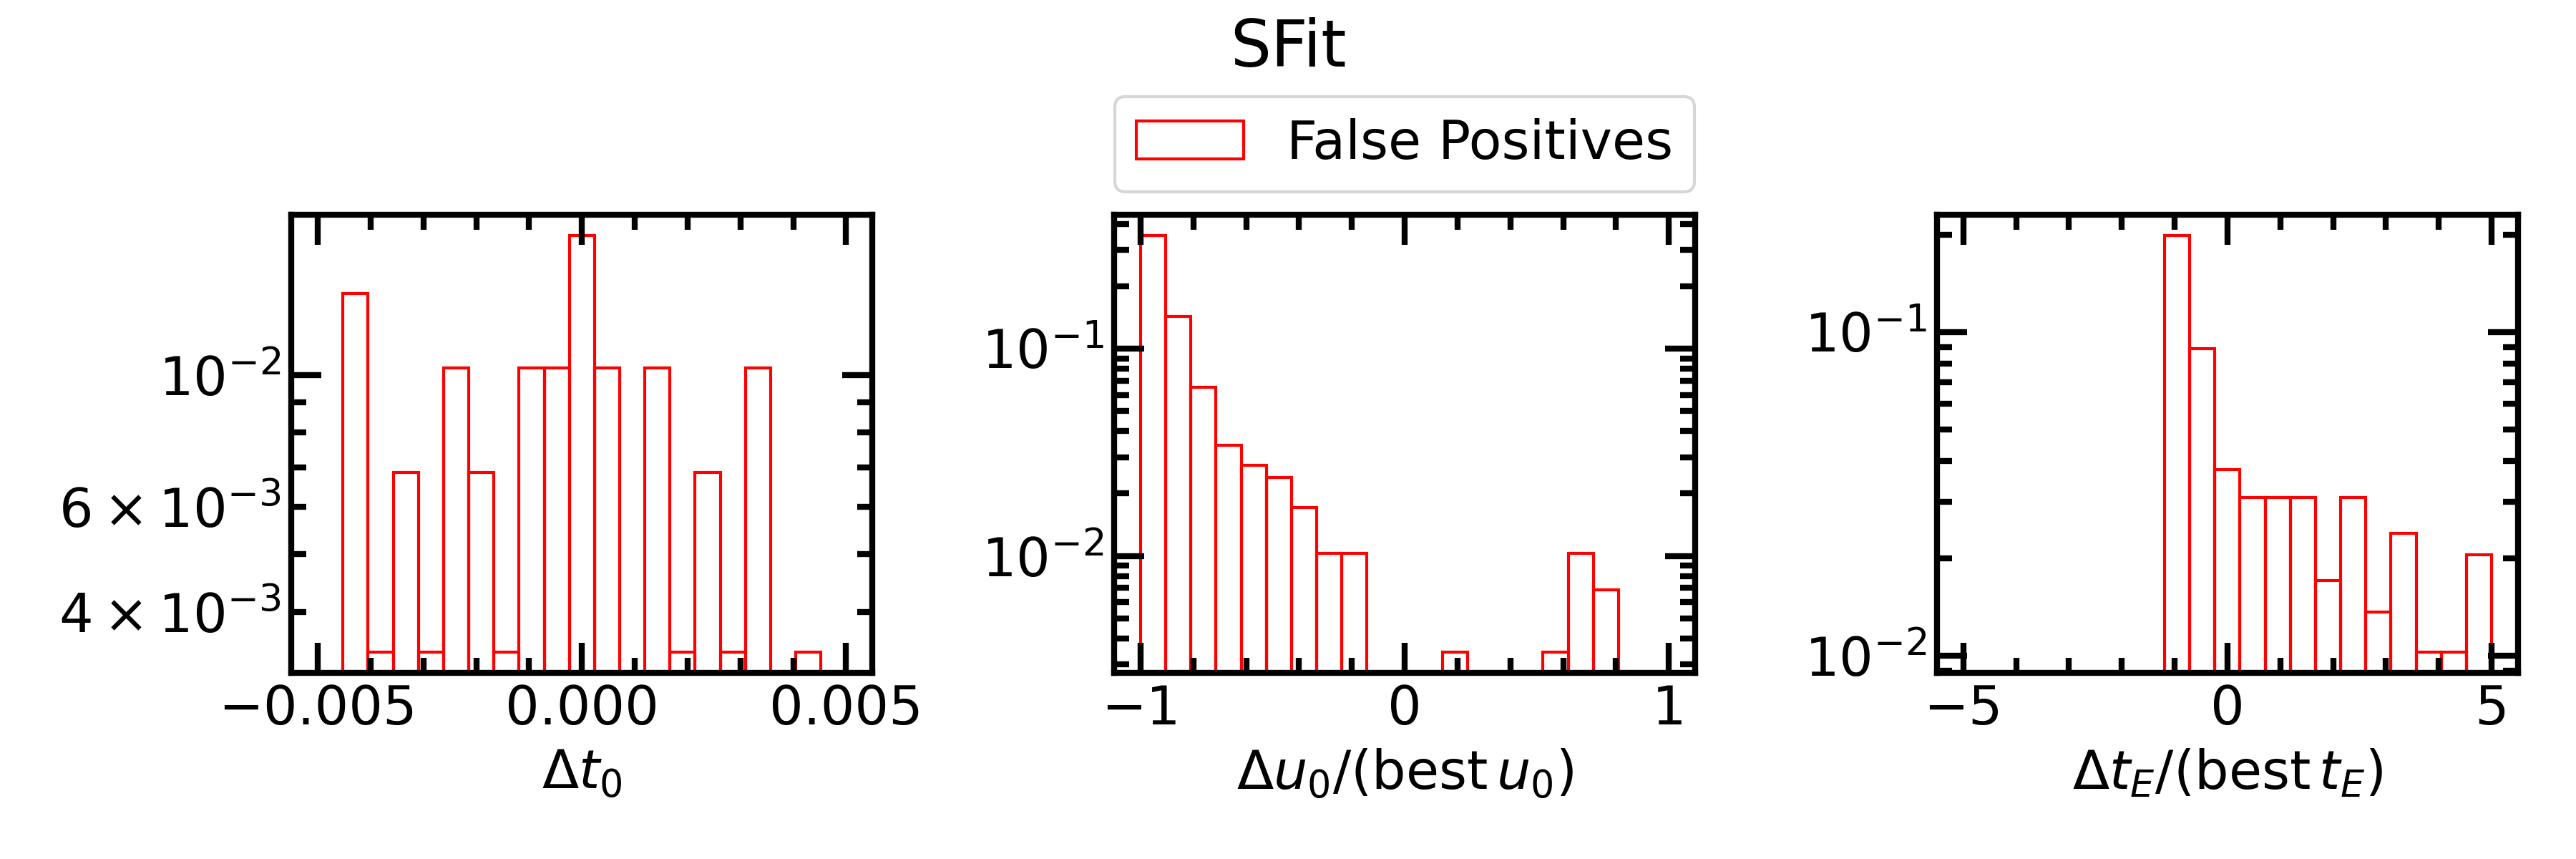
\includegraphics[width=\textwidth]{figs/hist_SFit.png}
	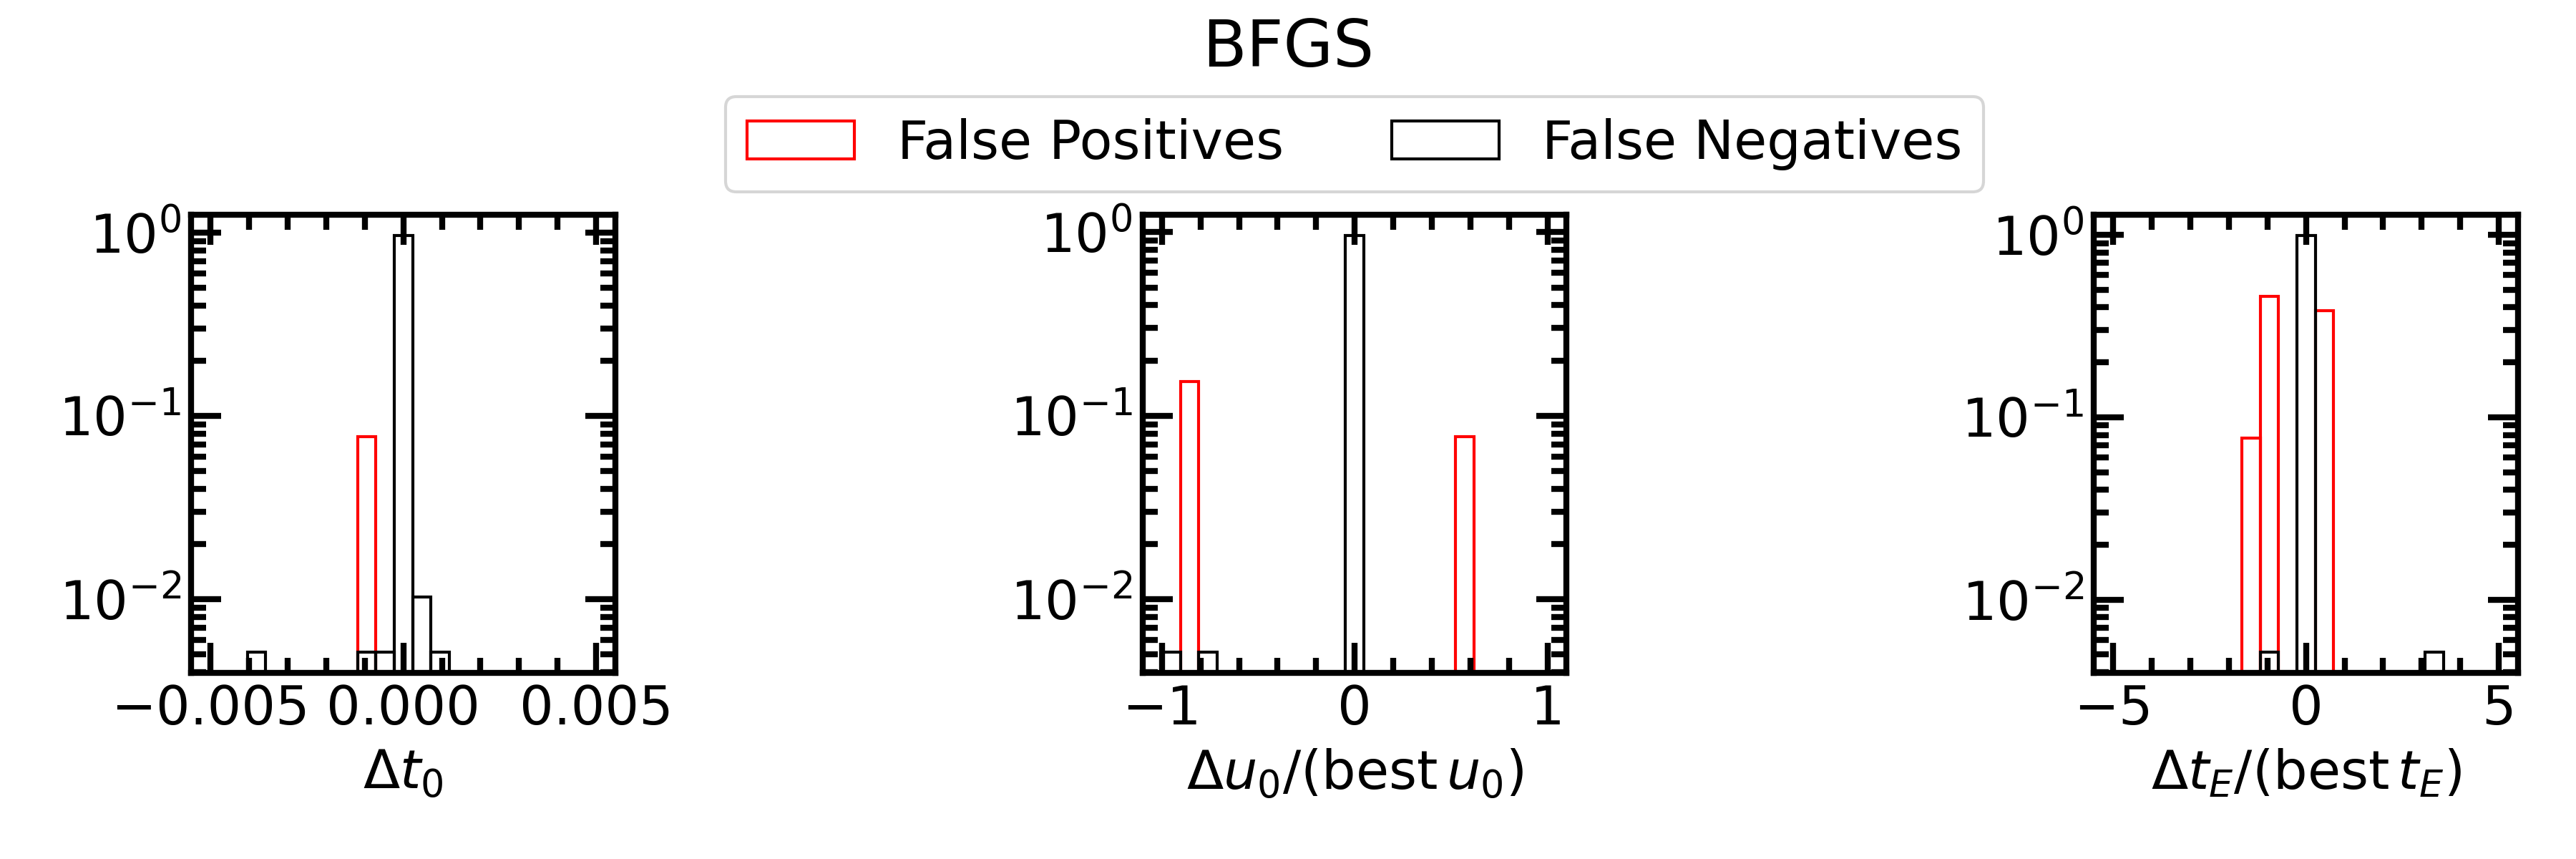
\includegraphics[width=\textwidth]{figs/hist_BFGS.png}
	\caption{\label{fig:hist}}
\end{figure}

\begin{deluxetable}{lrrrr}
\tablecaption{Number of $\chi^2$ Function Evalutions}
\label{tab:nfev}
\tablehead{
\colhead{Algorithm} & \colhead{Mean} &  \colhead{Median} &  \colhead{StdDev} &  \colhead{Max}
}
\startdata
\sfit            & 142.6 & 125 & 121.2 & 999\\
\neldarmead     & 348.8 & 303& 136.6 & 603\\
\newtoncg      & 44.5  & 21  & 80.2 & 633\\
\bfgs            & 122.1  & 44& 217.1 & 830\\
\enddata
\end{deluxetable}


\begin{comment}
\section{Gould Explanation}

Right, this might be a crucial difference.  "b" is defined in
"$\chi^2$ and linear fits", which is on arXiv
https://arxiv.org/pdf/astro-ph/0310577.pdf

The paper mainly describes linear fits, i.e., where the model
can be described by the equation just below section title
"Linear model" on page 2.

Then $b_{ij}$ is given by the second equation below "Minimizing $\chi^2$".

This is written in covariant formalism to allow for correlations
between the errors in the data points.  But for uncorrelated errors,
you can see from the in text equation after "In this case" on p2,
that ${B}_{kl} = \delta_{kl}/\sigma^2_k$.

So that, 
\begin{equation}
b_{ij} = \sum_k f_i(x_k)*f_j(x_k)/\sigma^2_k
\end{equation}
where $f_i(x)$ are the trial functions going into the linear fit.

You will notice that this is the same as in sfit, except that
instead of the $f_i(x)$ being linearized trial functions, they
are derivatives of the (nonlinear) trial functions.  I will get to
that.

Anyway, to continue with the linear problem for a bit, if we define
(for uncorrelated errors

\begin{eqnarray}
b_{ij} & = & \sum_k f_i(x_k)*f_j(x_k)/\sigma^2_k\\
d_i  & = & \sum_k f_i(x_k)*y_k/\sigma^2_k        \\     
\end{eqnarray}
where $y_k$ is the $k$-th data point.
then one can determine the linear coefficients $a_i$ by
\begin{equation}
a_i = \sum_j c_{ij} d_j   \quad\mathrm{where}\, c = b^{-1} \quad [3]
\end{equation}
(last two equations on p3).

OK, to relate what I have written here to "Newton's method"
(as discovered by Simpson), we need to consider two differences.
First, I am considering linear fits in many dimensions, and
Simpson is describing nonlinear fits it 1 dimension.

So, the difference that you identified between sfit and conventional
"Newton's method" really comes from two different paths to
bridging these TWO differences.  Before going into this, you
should look at the very short section "Nonlienar fits" on page 5,
which is the actual mathematical basis for sfit.

OK, for the general case, $\chi^2$ can be written as the first
equation under "Definition of $\chi^2$".  Then, for the linear
case, this equation can be written out explicitly as second
equation that follows (after "is written as").  This is just an
algebraic equations, which is soved by matrix inversion.

But going back to the general definition, and considering
the general (nonlinear) case, we can arrive at something similar
by Taylor expanding $\chi^2$, in terms of the n parameters.  I will
call these $A_i $(instead of $a_i$) as a reminder that in the general
case, they are non-linear
\begin{eqnarray}
\chi^2 & = &  \chi^2_0 + \sum_i {\partial \chi^2\over \partial A_i} A_i
+ {1\over2}\sum_{i,j} {\partial^2 \chi^22\over \partial A_i \partial A_j}A_i A_j\\
& = & \chi^2_0 + \sum_i D_i * A_i + \sum_{i,j} B_{ij} * A_i A_j  + ... \quad [4]
\end{eqnarray}
where
\begin{eqnarray}
D_i  & = & {\partial \chi^2\over \partial A_i}\\
B_{ij} & = & (1/2){\partial^2 \chi^2\over \partial A_i\partial A_j}  \quad [5]
\end{eqnarray}

So then this can be solved by (first ignoring higher order terms [4])
and then
\begin{equation}
A_i = -\sum_j C_{ij} D_j \quad               [6]
\end{equation}
which looks very similar to [3], except that Equation [5] is different
from Equation [2], i.e., it somehow now involves second derivatives.

Anyway, let's push ahead and evaluate [5] for the case of a linear function
$F(x) = \sum_i a_i f_i(x)$

Then
\begin{equation}
\partial \chi^2/\partial a_i = -2\sum_k (y_k - F(x_k))f_i(x_k)/\sigma^2_k
\end{equation}
and
\begin{equation}
\partial \chi^2/\partial a_i\partial a_j=
2\sum_k f_i(x_k)f_j(x_k)/\sigma^2_k
\end{equation}

That is, for the case of linear fits, the solution (derived from
second derivative of chi2) can be expressed
in terms of products of the FIRST derivatives of the general functional
form.  That is, the $\chi^2$ has a term $[F(x)]^2$, whose second derivative is
\begin{equation}
\partial^2 [F(x)]^2/\partial a_i \partial a_j =
F(x)\partial*2 F(x)/\partial a_i\partial a_j
+ 2\partial F(x)/\partial a_i\partial F(x)/\partial a_j
\end{equation}
But for the special case $F(x) = \sum_i a_i f_i(x)$
then
\begin{equation}
\partial F(x)/\partial a_i = f_i(x)
\end{equation}
and
\begin{equation}
\partial*2 F(x)/\partial a_i\partial a_j = 0,
\end{equation}
so the first term disappears.

Hence, there are three ways to generalize Simpson's idea
to mutliple dimenions.
1) use only first derivatives (which is what Simpson did in
   1-D), so-called gradient method
2) Taylor expand $\chi^2$ and truncate at second term, then
   solve this (very inexact equation) exactly by inversion
   of the matrix of second derivatives (Hessian)
3) first generalize Simpson's idea that a 1-D function is well
   described by it first derivative (which can easily be solved
   exactly) to several dimensions, i.e., the function is well
   described by a tangent plane.  And solve this exactly.

So, it is possible that the method that I developed is actually
"new".  That is, a different generalization of Simpson than
was previously known.   It could be better if derivatives are derived
numerically, because first derivatives are a lot more stable than
second derivatives.

\end{comment}

%
%\begin{thebibliography}{999}
%\bibitem[Gould(2003)]{Gould03} Gould, A.\ 2003, astro-ph/0310577
%\end{thebibliography}

\end{document}